\chapter{Estratégias de Abordagem aos Problemas} \label{cap:abordagem}
Nesta secção vamos analisar os procedimentos, tecnologias e conceitos utilizados no desenvolvimento deste projeto.

\section{Modelo de Dados} \label{sec:dados}
Um dos componentes deste sistema é um repositório de dados, que irá conter as várias informações relacionadas com os clientes deste serviço. Na figura \ref{fig:relacoes} estão representados os vários elementos deste modelo de dados. \\
O elemento utilizador representa um utilizador do sistema. Para cada utilizador será registado um ID único, o seu nome, email e número de telefone/telemóvel. Os utilizadores podem ser utilizadores administradores ou podem ser clientes. Os clientes, para além dos dados registados como utilizador, têm também o seu número de cliente e número de conta e a sua morada. \\
Os utilizadores terão associado um ou mais contadores, pelo que para cada contador guardamos o seu número único de instalação, o seu número de série, o cliente e o contrato ao qual ele está associado, a sua última medição e o local onde está em utilização. \\
As várias contagens efetuadas também estarão guardadas, associadas a cada contador. Cada contagem será identificada pelo número da fatura correspondente ao pagamento dessa contagem e também será armazenado o tipo de cliente ou tarifa referente. \\
Por fim, cada contagem tem um custo associado, que é composto pelo custo da água consumida, pelo custo do saneamento, pelo custo de tratamento de resíduos sólidos e as várias taxas e IVA inerentes ao pagamento deste serviço.

\begin{figure}[ht!]
\centering
\resizebox{110mm}{!}{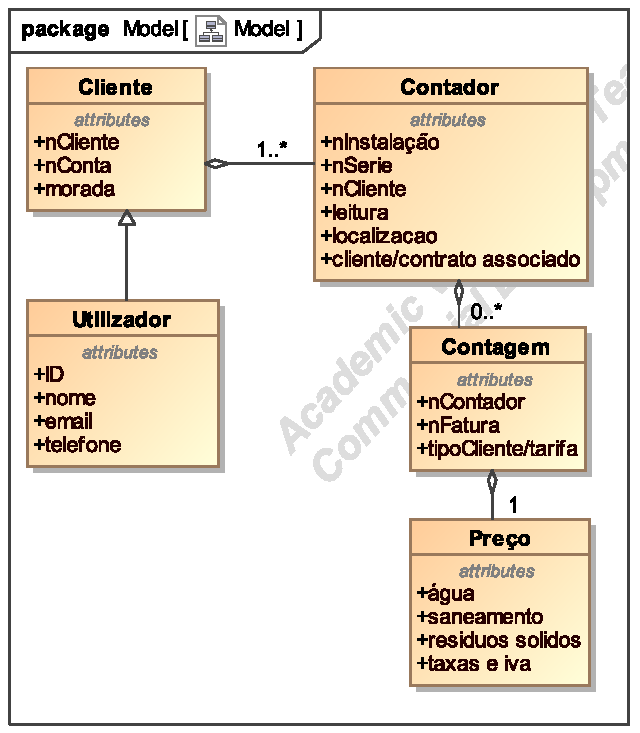
\includegraphics{diagramas/svg/uml__Model.pdf}}
\caption{Arquitetura do sistema.}
\label{fig:relacoes}
\end{figure}